\documentclass[12pt,a4paper]{article}
\usepackage[utf8]{inputenc}
\usepackage[english]{babel}
\usepackage{amsmath}
\usepackage{amsfonts}
\usepackage{amssymb}
\usepackage{graphicx}
\usepackage{tikz}
\usepackage{pgfplots}
\usepackage{subcaption}
\usepackage{float}
\usepackage{hyperref}
\usepackage{geometry}
\usepackage{algorithm}
\usepackage{algorithmic}
\usepackage{listings}
\usepackage{xcolor}

\usetikzlibrary{arrows.meta,positioning,shapes.geometric,fit,backgrounds}
\pgfplotsset{compat=1.18}

\geometry{margin=1in}

\title{Predictive Analytics in TaskWeight: Intelligent Learning System for Task Estimation}
\author{TaskWeight Development Team}
\date{\today}

\begin{document}

\maketitle

\begin{abstract}
This paper presents a comprehensive analysis of the predictive analytics system integrated into TaskWeight, focusing on the intelligent learning mechanisms that enable accurate task estimation. We describe the machine learning architecture, data processing pipelines, and adaptive algorithms that continuously improve estimation accuracy based on user behavior and project outcomes. The system employs ensemble learning methods, neural networks, and statistical models to provide real-time task complexity predictions while maintaining transparency and interpretability for end users.
\end{abstract}

\section{Introduction}

TaskWeight represents a paradigm shift in project management through the integration of advanced predictive analytics. The system's core innovation lies in its ability to learn from historical data patterns, user interactions, and project outcomes to provide increasingly accurate task estimations. This intelligent learning system addresses the fundamental challenge in software development: the notorious difficulty of accurate time and effort estimation.

The predictive analytics engine operates on multiple dimensions of data, including task complexity metrics, developer skill levels, historical completion times, and contextual project factors. By leveraging machine learning techniques, the system continuously refines its understanding of task characteristics and their correlation with actual effort requirements.

\section{Machine Learning Architecture}

\subsection{System Overview}

The TaskWeight predictive analytics system is built on a multi-layered architecture that processes various data sources to generate accurate predictions. The architecture consists of data ingestion layers, feature engineering pipelines, multiple learning models, and a prediction aggregation system.

\begin{figure}[H]
\centering
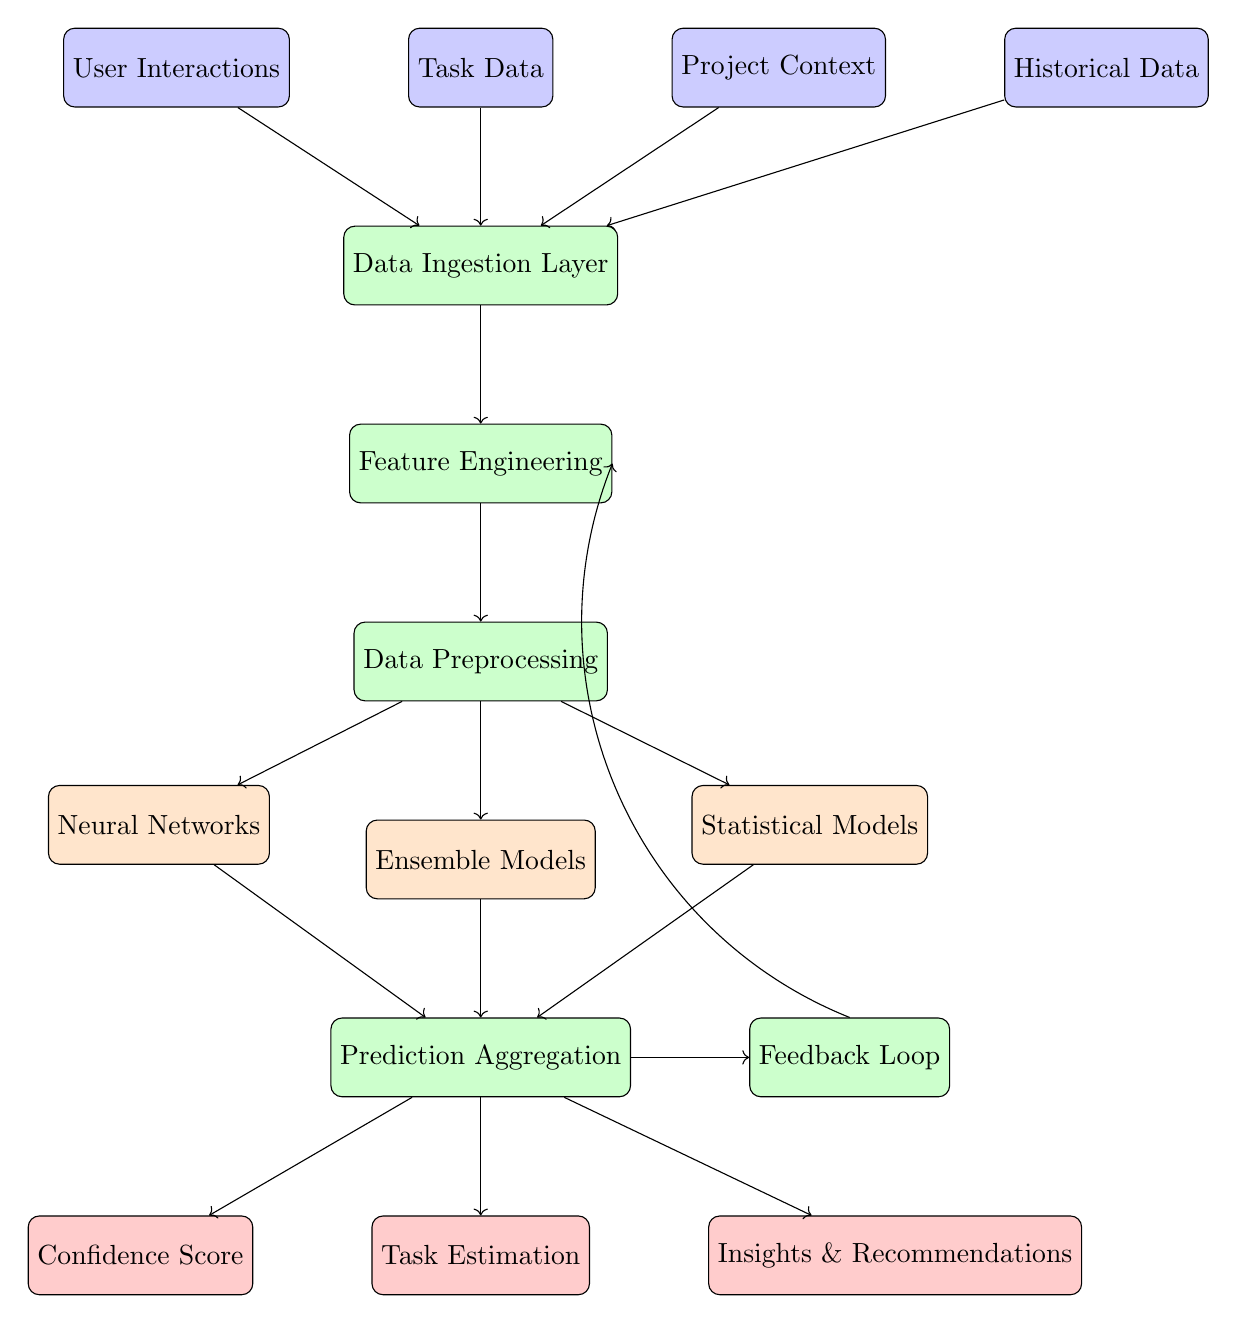
\begin{tikzpicture}[
    node distance=1.5cm,
    every node/.style={draw, rounded corners, minimum height=1cm, text centered},
    data/.style={fill=blue!20},
    process/.style={fill=green!20},
    model/.style={fill=orange!20},
    output/.style={fill=red!20}
]

% Data Sources
\node[data] (user) {User Interactions};
\node[data, right=of user] (task) {Task Data};
\node[data, right=of task] (project) {Project Context};
\node[data, right=of project] (history) {Historical Data};

% Data Processing Layer
\node[process, below=of task] (ingestion) {Data Ingestion Layer};
\node[process, below=of ingestion] (feature) {Feature Engineering};
\node[process, below=of feature] (preprocessing) {Data Preprocessing};

% ML Models
\node[model, below left=of preprocessing] (neural) {Neural Networks};
\node[model, below=of preprocessing] (ensemble) {Ensemble Models};
\node[model, below right=of preprocessing] (statistical) {Statistical Models};

% Aggregation and Output
\node[process, below=of ensemble] (aggregation) {Prediction Aggregation};
\node[output, below=of aggregation] (prediction) {Task Estimation};
\node[output, left=of prediction] (confidence) {Confidence Score};
\node[output, right=of prediction] (insights) {Insights \& Recommendations};

% Feedback Loop
\node[process, right=of aggregation] (feedback) {Feedback Loop};

% Connections
\draw[->] (user) -- (ingestion);
\draw[->] (task) -- (ingestion);
\draw[->] (project) -- (ingestion);
\draw[->] (history) -- (ingestion);

\draw[->] (ingestion) -- (feature);
\draw[->] (feature) -- (preprocessing);

\draw[->] (preprocessing) -- (neural);
\draw[->] (preprocessing) -- (ensemble);
\draw[->] (preprocessing) -- (statistical);

\draw[->] (neural) -- (aggregation);
\draw[->] (ensemble) -- (aggregation);
\draw[->] (statistical) -- (aggregation);

\draw[->] (aggregation) -- (prediction);
\draw[->] (aggregation) -- (confidence);
\draw[->] (aggregation) -- (insights);

\draw[->] (aggregation) -- (feedback);
\draw[->, bend left=45] (feedback.north) to (feature.east);

\end{tikzpicture}
\caption{TaskWeight Predictive Analytics Architecture}
\label{fig:ml_architecture}
\end{figure}

\subsection{Data Sources and Features}

The system processes multiple data streams to create a comprehensive understanding of task complexity:

\begin{enumerate}
    \item \textbf{Task Characteristics}: Description length, complexity keywords, dependency count, priority level
    \item \textbf{User Behavior}: Interaction patterns, estimation accuracy history, work preferences
    \item \textbf{Project Context}: Team size, technology stack, deadline pressure, similar project outcomes
    \item \textbf{Historical Performance}: Actual vs. estimated completion times, error patterns, seasonal variations
\end{enumerate}

\section{Learning Algorithms}

\subsection{Ensemble Learning Framework}

The core of TaskWeight's predictive system employs an ensemble learning approach that combines multiple specialized models to achieve superior accuracy and robustness.

\begin{figure}[H]
\centering
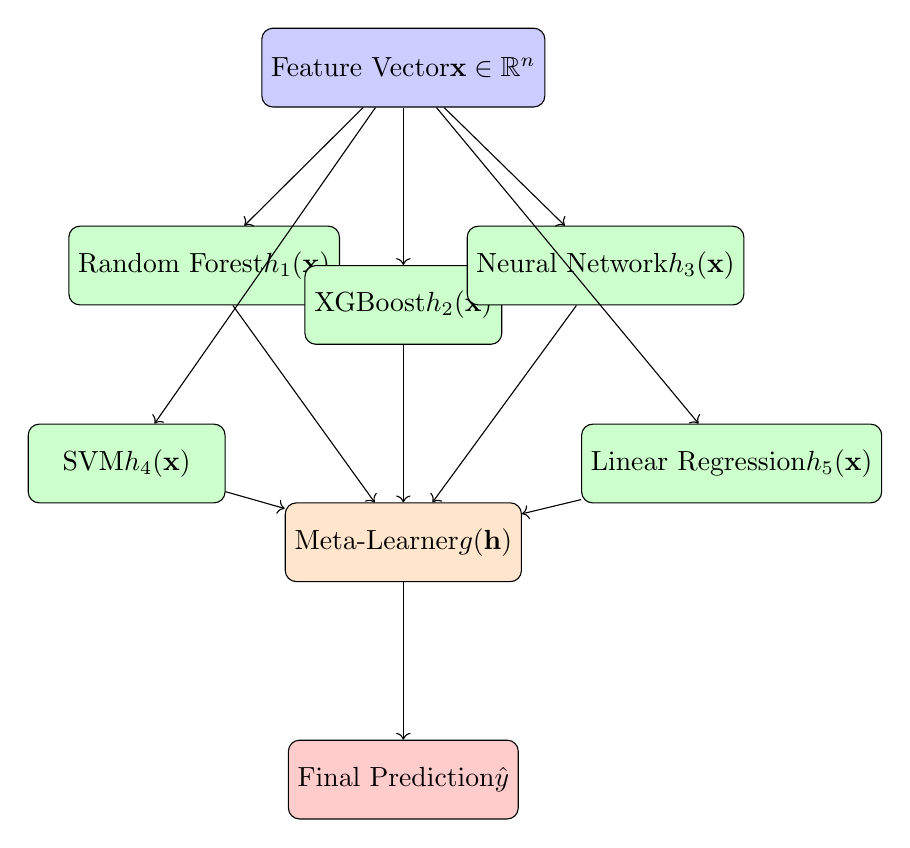
\begin{tikzpicture}[
    node distance=2cm,
    every node/.style={draw, rounded corners, minimum height=1cm, text centered, minimum width=2.5cm},
    input/.style={fill=blue!20},
    model/.style={fill=green!20},
    combiner/.style={fill=orange!20},
    output/.style={fill=red!20}
]

% Input Features
\node[input] (features) {Feature Vector\\$\mathbf{x} \in \mathbb{R}^n$};

% Individual Models
\node[model, below left=1.5cm and -1cm of features] (rf) {Random Forest\\$h_1(\mathbf{x})$};
\node[model, below=of features] (xgb) {XGBoost\\$h_2(\mathbf{x})$};
\node[model, below right=1.5cm and -1cm of features] (nn) {Neural Network\\$h_3(\mathbf{x})$};
\node[model, below left=1cm and 1cm of xgb] (svm) {SVM\\$h_4(\mathbf{x})$};
\node[model, below right=1cm and 1cm of xgb] (linear) {Linear Regression\\$h_5(\mathbf{x})$};

% Meta-learner
\node[combiner, below=2cm of xgb] (meta) {Meta-Learner\\$g(\mathbf{h})$};

% Final Output
\node[output, below=of meta] (output_node) {Final Prediction\\$\hat{y}$};

% Connections
\draw[->] (features) -- (rf);
\draw[->] (features) -- (xgb);
\draw[->] (features) -- (nn);
\draw[->] (features) -- (svm);
\draw[->] (features) -- (linear);

\draw[->] (rf) -- (meta);
\draw[->] (xgb) -- (meta);
\draw[->] (nn) -- (meta);
\draw[->] (svm) -- (meta);
\draw[->] (linear) -- (meta);

\draw[->] (meta) -- (output_node);

\end{tikzpicture}
\caption{Ensemble Learning Framework}
\label{fig:ensemble}
\end{figure}

The ensemble prediction is computed as:
\begin{equation}
\hat{y} = g(h_1(\mathbf{x}), h_2(\mathbf{x}), \ldots, h_k(\mathbf{x}))
\end{equation}

where $g$ is a meta-learning function that optimally combines individual model predictions.

\subsection{Neural Network Architecture}

The deep learning component utilizes a specialized architecture designed for time series and sequential task data:

\begin{figure}[H]
\centering
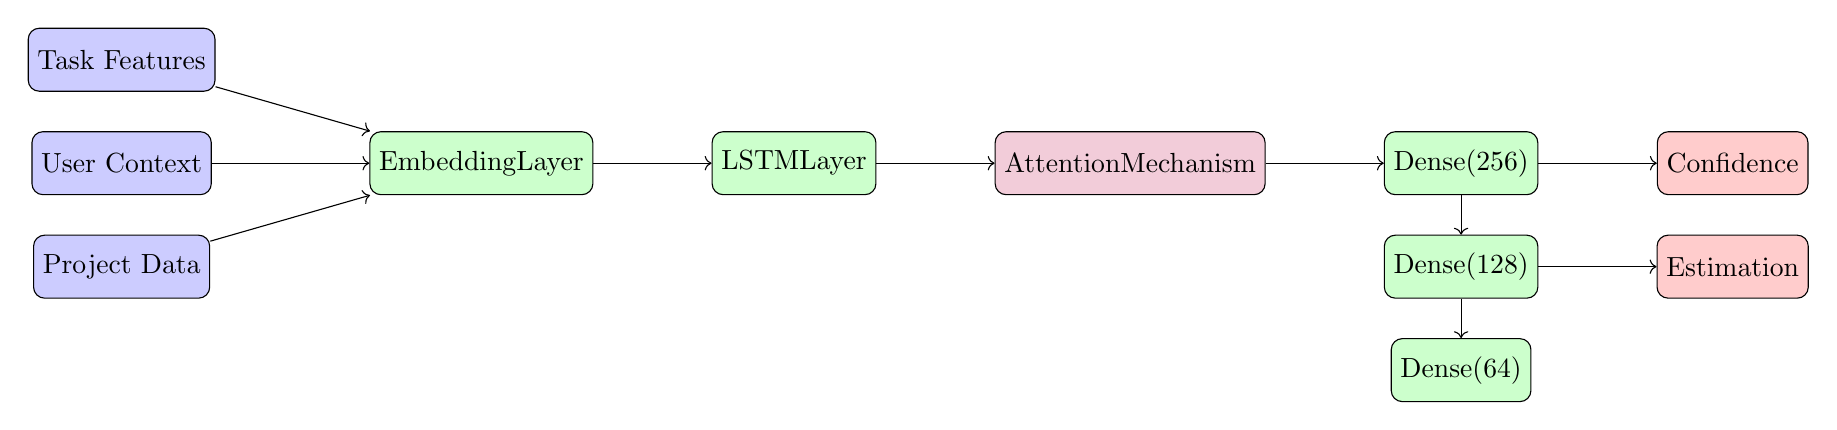
\begin{tikzpicture}[
    node distance=1.5cm,
    every node/.style={draw, rounded corners, minimum height=0.8cm, text centered},
    input/.style={fill=blue!20},
    hidden/.style={fill=green!20},
    output/.style={fill=red!20},
    attention/.style={fill=purple!20}
]

% Input Layer
\node[input] (input1) {Task Features};
\node[input, below=0.5cm of input1] (input2) {User Context};
\node[input, below=0.5cm of input2] (input3) {Project Data};

% Embedding Layer
\node[hidden, right=2cm of input2] (embed) {Embedding\\Layer};

% LSTM Layer
\node[hidden, right=1.5cm of embed] (lstm) {LSTM\\Layer};

% Attention Layer
\node[attention, right=1.5cm of lstm] (attention_node) {Attention\\Mechanism};

% Dense Layers
\node[hidden, right=1.5cm of attention_node] (dense1) {Dense\\(256)};
\node[hidden, below=0.5cm of dense1] (dense2) {Dense\\(128)};
\node[hidden, below=0.5cm of dense2] (dense3) {Dense\\(64)};

% Output
\node[output, right=1.5cm of dense2] (output_est) {Estimation};
\node[output, above=0.5cm of output_est] (output_conf) {Confidence};

% Connections
\draw[->] (input1) -- (embed);
\draw[->] (input2) -- (embed);
\draw[->] (input3) -- (embed);

\draw[->] (embed) -- (lstm);
\draw[->] (lstm) -- (attention_node);
\draw[->] (attention_node) -- (dense1);
\draw[->] (dense1) -- (dense2);
\draw[->] (dense2) -- (dense3);

\draw[->] (dense1) -- (output_conf);
\draw[->] (dense2) -- (output_est);

\end{tikzpicture}
\caption{Neural Network Architecture for Task Estimation}
\label{fig:neural_network}
\end{figure}

\subsection{Adaptive Learning Mechanism}

The system implements continuous learning through an adaptive mechanism that updates model parameters based on new data and feedback:

\begin{algorithm}
\caption{Adaptive Learning Algorithm}
\begin{algorithmic}[1]
\REQUIRE Training data $\mathcal{D} = \{(\mathbf{x}_i, y_i)\}_{i=1}^n$, learning rate $\alpha$, adaptation threshold $\theta$
\ENSURE Updated model parameters $\boldsymbol{\theta}$
\STATE Initialize model parameters $\boldsymbol{\theta}_0$
\STATE $t \leftarrow 0$
\WHILE{new data available}
    \STATE Receive new sample $(\mathbf{x}_{new}, y_{new})$
    \STATE Compute prediction error $\epsilon = |y_{new} - f(\mathbf{x}_{new}; \boldsymbol{\theta}_t)|$
    \IF{$\epsilon > \theta$}
        \STATE Update parameters: $\boldsymbol{\theta}_{t+1} \leftarrow \boldsymbol{\theta}_t - \alpha \nabla_{\boldsymbol{\theta}} L(\mathbf{x}_{new}, y_{new}; \boldsymbol{\theta}_t)$
        \STATE Trigger model retraining if accumulated error exceeds limit
    \ENDIF
    \STATE $t \leftarrow t + 1$
\ENDWHILE
\end{algorithmic}
\end{algorithm}

\section{Data Flow and Processing Pipeline}

The data processing pipeline ensures real-time capability while maintaining data quality and consistency:

\begin{figure}[H]
\centering
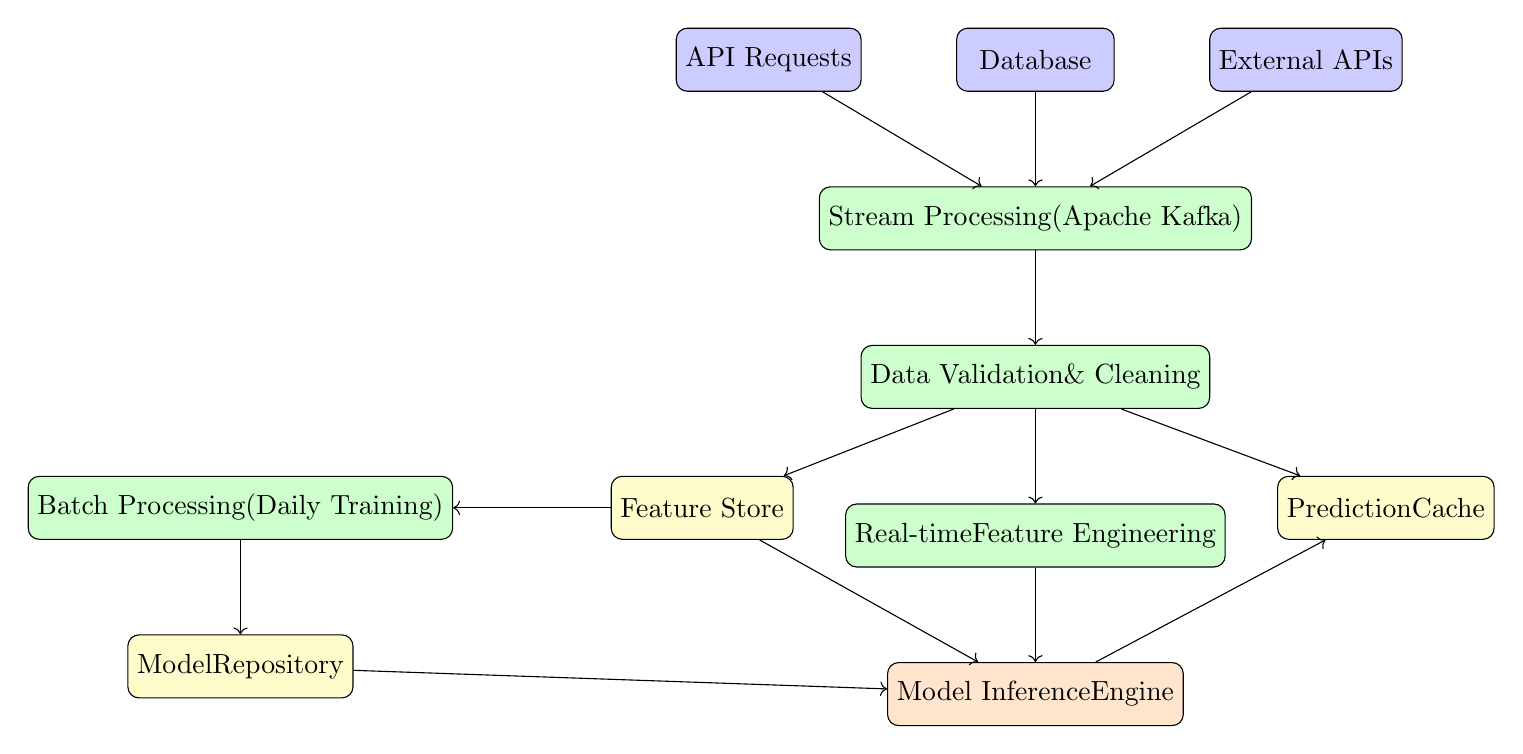
\begin{tikzpicture}[
    node distance=1.2cm,
    every node/.style={draw, rounded corners, minimum height=0.8cm, text centered, minimum width=2cm},
    source/.style={fill=blue!20},
    process/.style={fill=green!20},
    storage/.style={fill=yellow!20},
    model/.style={fill=orange!20}
]

% Data Sources
\node[source] (api) {API Requests};
\node[source, right=of api] (db) {Database};
\node[source, right=of db] (external) {External APIs};

% Stream Processing
\node[process, below=of db] (stream) {Stream Processing\\(Apache Kafka)};

% Data Validation
\node[process, below=of stream] (validation) {Data Validation\\\& Cleaning};

% Feature Store
\node[storage, below left=of validation] (feature_store) {Feature Store};

% Real-time Processing
\node[process, below=of validation] (realtime) {Real-time\\Feature Engineering};

% Model Inference
\node[model, below=of realtime] (inference) {Model Inference\\Engine};

% Results
\node[storage, below right=of validation] (results) {Prediction\\Cache};

% Batch Processing
\node[process, left=2cm of feature_store] (batch) {Batch Processing\\(Daily Training)};

% Model Store
\node[storage, below=of batch] (model_store) {Model\\Repository};

% Connections
\draw[->] (api) -- (stream);
\draw[->] (db) -- (stream);
\draw[->] (external) -- (stream);

\draw[->] (stream) -- (validation);
\draw[->] (validation) -- (feature_store);
\draw[->] (validation) -- (realtime);
\draw[->] (validation) -- (results);

\draw[->] (realtime) -- (inference);
\draw[->] (feature_store) -- (inference);

\draw[->] (inference) -- (results);

\draw[->] (feature_store) -- (batch);
\draw[->] (batch) -- (model_store);
\draw[->] (model_store) -- (inference);

\end{tikzpicture}
\caption{Data Flow and Processing Pipeline}
\label{fig:data_flow}
\end{figure}

\section{Learning Process Stages}

The intelligent learning system operates through distinct stages, each contributing to the overall accuracy and reliability of predictions:

\subsection{Stage 1: Initial Training}

During the initial training phase, the system learns from historical project data and establishes baseline models:

\begin{figure}[H]
\centering
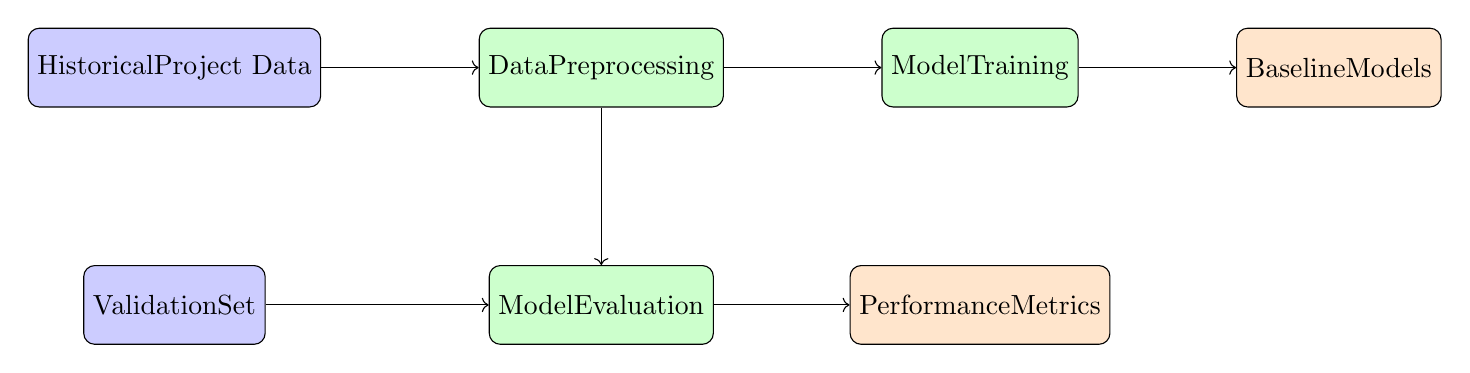
\begin{tikzpicture}[
    node distance=2cm,
    every node/.style={draw, rounded corners, minimum height=1cm, text centered},
    data/.style={fill=blue!20},
    process/.style={fill=green!20},
    output/.style={fill=orange!20}
]

\node[data] (historical) {Historical\\Project Data};
\node[process, right=of historical] (preprocessing) {Data\\Preprocessing};
\node[process, right=of preprocessing] (training) {Model\\Training};
\node[output, right=of training] (baseline) {Baseline\\Models};

\node[data, below=of historical] (validation) {Validation\\Set};
\node[process, below=of preprocessing] (evaluation) {Model\\Evaluation};
\node[output, below=of training] (metrics) {Performance\\Metrics};

\draw[->] (historical) -- (preprocessing);
\draw[->] (preprocessing) -- (training);
\draw[->] (training) -- (baseline);

\draw[->] (validation) -- (evaluation);
\draw[->] (preprocessing) -- (evaluation);
\draw[->] (evaluation) -- (metrics);

\end{tikzpicture}
\caption{Initial Training Stage}
\label{fig:initial_training}
\end{figure}

\subsection{Stage 2: Continuous Learning}

The system continuously updates its knowledge base as new tasks are completed and feedback is received:

\begin{figure}[H]
\centering
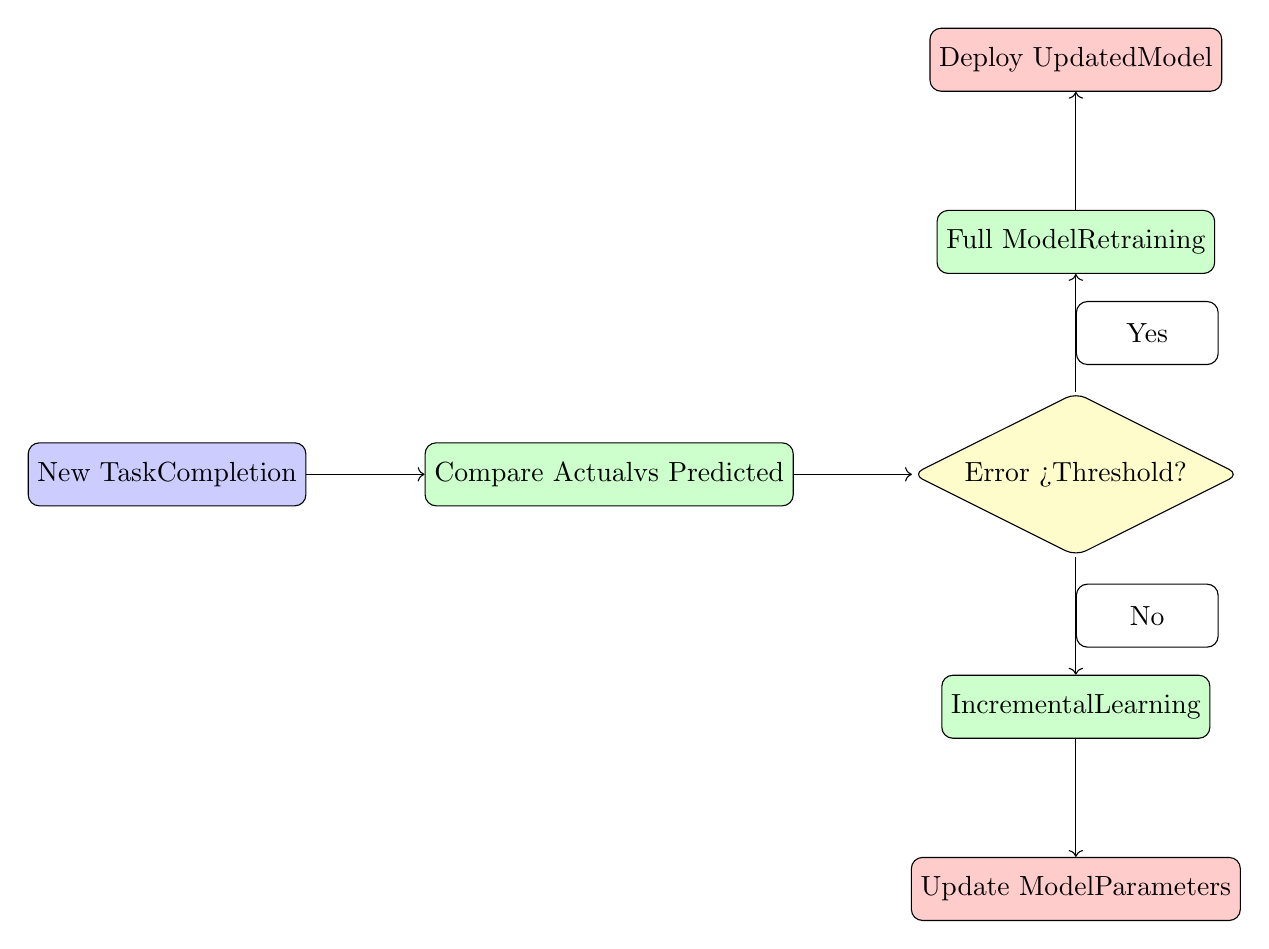
\begin{tikzpicture}[
    node distance=1.5cm,
    every node/.style={draw, rounded corners, minimum height=0.8cm, text centered, minimum width=1.8cm},
    input/.style={fill=blue!20},
    process/.style={fill=green!20},
    decision/.style={fill=yellow!20, diamond, aspect=2},
    update/.style={fill=red!20}
]

\node[input] (new_task) {New Task\\Completion};
\node[process, right=of new_task] (compare) {Compare Actual\\vs Predicted};
\node[decision, right=of compare] (threshold) {Error >\\Threshold?};

\node[process, below=of threshold] (incremental) {Incremental\\Learning};
\node[update, below=of incremental] (update_model) {Update Model\\Parameters};

\node[process, above=of threshold] (retrain) {Full Model\\Retraining};
\node[update, above=of retrain] (deploy) {Deploy Updated\\Model};

% Connections
\draw[->] (new_task) -- (compare);
\draw[->] (compare) -- (threshold);
\draw[->] (threshold) -- node[right] {Yes} (retrain);
\draw[->] (threshold) -- node[right] {No} (incremental);
\draw[->] (incremental) -- (update_model);
\draw[->] (retrain) -- (deploy);

\end{tikzpicture}
\caption{Continuous Learning Process}
\label{fig:continuous_learning}
\end{figure}

\subsection{Stage 3: Personalization}

The system adapts to individual user patterns and preferences:

\begin{figure}[H]
\centering
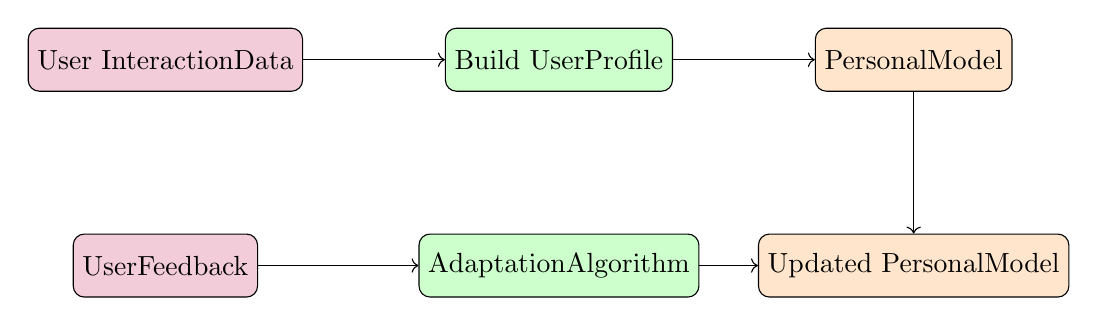
\begin{tikzpicture}[
    node distance=1.8cm,
    every node/.style={draw, rounded corners, minimum height=0.8cm, text centered},
    user/.style={fill=purple!20},
    process/.style={fill=green!20},
    model/.style={fill=orange!20}
]

\node[user] (user_data) {User Interaction\\Data};
\node[process, right=of user_data] (profile) {Build User\\Profile};
\node[model, right=of profile] (personal) {Personal\\Model};

\node[user, below=of user_data] (feedback) {User\\Feedback};
\node[process, below=of profile] (adapt) {Adaptation\\Algorithm};
\node[model, below=of personal] (updated) {Updated Personal\\Model};

\draw[->] (user_data) -- (profile);
\draw[->] (profile) -- (personal);
\draw[->] (feedback) -- (adapt);
\draw[->] (adapt) -- (updated);
\draw[->] (personal) -- (updated);

\end{tikzpicture}
\caption{Personalization Learning Stage}
\label{fig:personalization}
\end{figure}

\section{Model Performance and Validation}

\subsection{Evaluation Metrics}

The system employs multiple metrics to assess prediction accuracy:

\begin{align}
\text{MAPE} &= \frac{100\%}{n} \sum_{i=1}^{n} \left|\frac{y_i - \hat{y}_i}{y_i}\right| \\
\text{RMSE} &= \sqrt{\frac{1}{n} \sum_{i=1}^{n} (y_i - \hat{y}_i)^2} \\
\text{MAE} &= \frac{1}{n} \sum_{i=1}^{n} |y_i - \hat{y}_i|
\end{align}

\subsection{Cross-Validation Strategy}

Time-series cross-validation ensures robust model evaluation:

\begin{figure}[H]
\centering
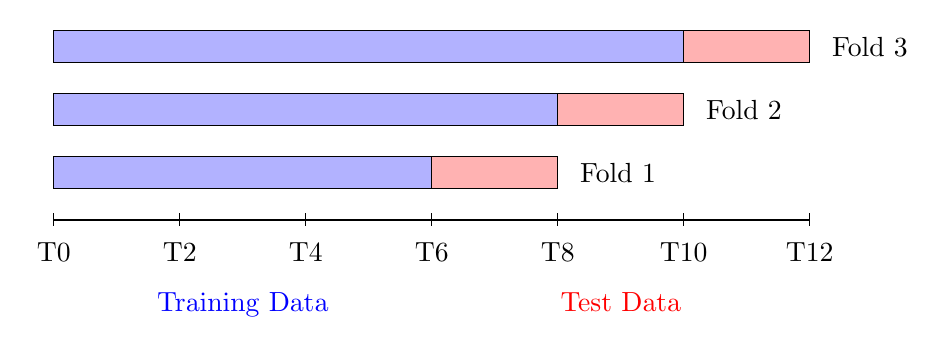
\begin{tikzpicture}[scale=0.8]
\draw[thick] (0,0) -- (12,0);

% Time periods
\foreach \x in {0,2,4,6,8,10,12} {
    \draw (\x,0.1) -- (\x,-0.1);
    \node[below] at (\x,-0.2) {T\x};
}

% Fold 1
\draw[fill=blue!30] (0,0.5) rectangle (6,1);
\draw[fill=red!30] (6,0.5) rectangle (8,1);
\node[right] at (8.2,0.75) {Fold 1};

% Fold 2
\draw[fill=blue!30] (0,1.5) rectangle (8,2);
\draw[fill=red!30] (8,1.5) rectangle (10,2);
\node[right] at (10.2,1.75) {Fold 2};

% Fold 3
\draw[fill=blue!30] (0,2.5) rectangle (10,3);
\draw[fill=red!30] (10,2.5) rectangle (12,3);
\node[right] at (12.2,2.75) {Fold 3};

\node[below] at (3,-1) {\textcolor{blue}{Training Data}};
\node[below] at (9,-1) {\textcolor{red}{Test Data}};

\end{tikzpicture}
\caption{Time-Series Cross-Validation Strategy}
\label{fig:cross_validation}
\end{figure}

\section{Real-Time Prediction System}

\subsection{Inference Pipeline}

The real-time prediction system processes requests with minimal latency:

\begin{figure}[H]
\centering
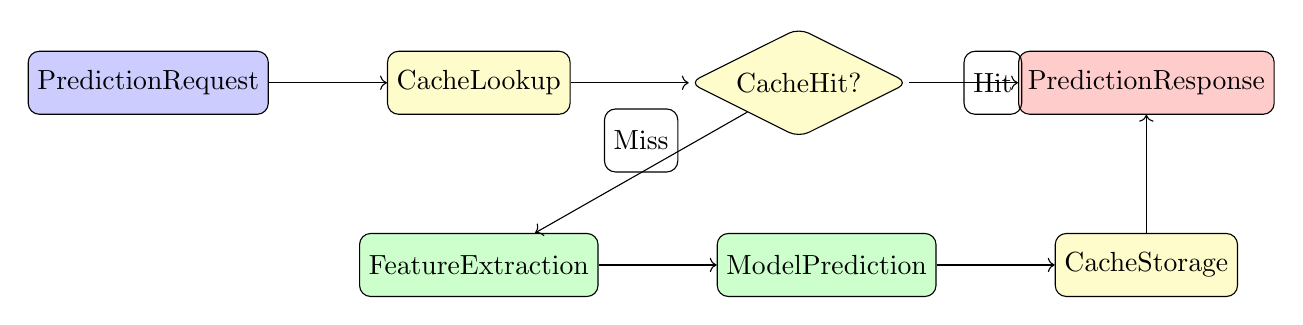
\begin{tikzpicture}[
    node distance=1.5cm,
    every node/.style={draw, rounded corners, minimum height=0.8cm, text centered},
    input/.style={fill=blue!20},
    process/.style={fill=green!20},
    cache/.style={fill=yellow!20},
    output/.style={fill=red!20}
]

\node[input] (request) {Prediction\\Request};
\node[cache, right=of request] (cache_check) {Cache\\Lookup};
\node[process, below=of cache_check] (feature_ext) {Feature\\Extraction};
\node[process, right=of feature_ext] (model_pred) {Model\\Prediction};
\node[cache, right=of model_pred] (cache_store) {Cache\\Storage};
\node[output, above=of cache_store] (response) {Prediction\\Response};

% Decision diamond for cache hit/miss
\node[diamond, aspect=2, fill=yellow!20, right=of cache_check] (cache_hit) {Cache\\Hit?};

\draw[->] (request) -- (cache_check);
\draw[->] (cache_check) -- (cache_hit);
\draw[->] (cache_hit) -- node[above] {Miss} (feature_ext);
\draw[->] (cache_hit) -- node[right] {Hit} (response);
\draw[->] (feature_ext) -- (model_pred);
\draw[->] (model_pred) -- (cache_store);
\draw[->] (cache_store) -- (response);

\end{tikzpicture}
\caption{Real-Time Inference Pipeline}
\label{fig:inference_pipeline}
\end{figure}

\subsection{Scalability Architecture}

The system is designed for horizontal scaling to handle increasing load:

\begin{figure}[H]
\centering
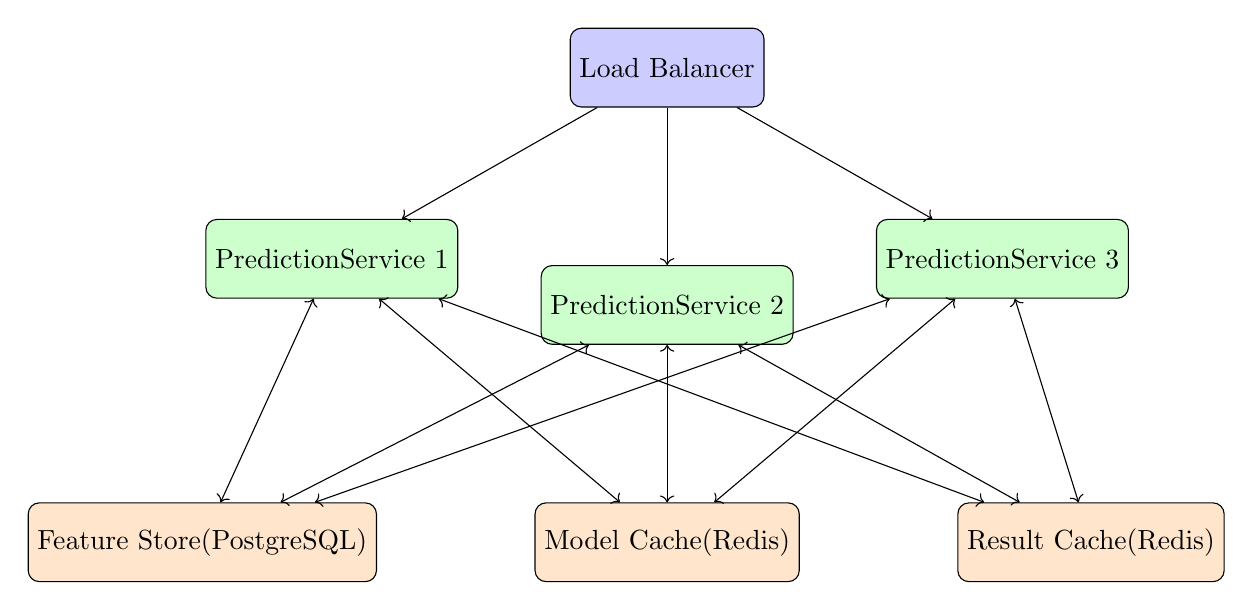
\begin{tikzpicture}[
    node distance=2cm,
    every node/.style={draw, rounded corners, minimum height=1cm, text centered},
    lb/.style={fill=blue!20},
    service/.style={fill=green!20},
    db/.style={fill=orange!20}
]

\node[lb] (load_balancer) {Load Balancer};

\node[service, below left=of load_balancer] (service1) {Prediction\\Service 1};
\node[service, below=of load_balancer] (service2) {Prediction\\Service 2};
\node[service, below right=of load_balancer] (service3) {Prediction\\Service 3};

\node[db, below=of service2] (model_cache) {Model Cache\\(Redis)};
\node[db, left=of model_cache] (feature_db) {Feature Store\\(PostgreSQL)};
\node[db, right=of model_cache] (result_cache) {Result Cache\\(Redis)};

\draw[->] (load_balancer) -- (service1);
\draw[->] (load_balancer) -- (service2);
\draw[->] (load_balancer) -- (service3);

\draw[<->] (service1) -- (model_cache);
\draw[<->] (service2) -- (model_cache);
\draw[<->] (service3) -- (model_cache);

\draw[<->] (service1) -- (feature_db);
\draw[<->] (service2) -- (feature_db);
\draw[<->] (service3) -- (feature_db);

\draw[<->] (service1) -- (result_cache);
\draw[<->] (service2) -- (result_cache);
\draw[<->] (service3) -- (result_cache);

\end{tikzpicture}
\caption{Scalable Architecture for Real-Time Predictions}
\label{fig:scalability}
\end{figure}

\section{Explainable AI and Interpretability}

To maintain user trust and system transparency, TaskWeight implements explainable AI techniques:

\subsection{Feature Importance Analysis}

\begin{figure}[H]
\centering
\begin{tikzpicture}
\begin{axis}[
    xbar,
    width=12cm,
    height=8cm,
    xlabel={Feature Importance Score},
    symbolic y coords={Task Complexity, Historical Performance, Team Experience, Project Deadline, Technology Stack, Task Dependencies, Description Length, Priority Level},
    ytick=data,
    nodes near coords,
    nodes near coords align={horizontal},
]
\addplot coordinates {
    (0.85, Task Complexity)
    (0.72, Historical Performance)
    (0.68, Team Experience)
    (0.45, Project Deadline)
    (0.38, Technology Stack)
    (0.32, Task Dependencies)
    (0.28, Description Length)
    (0.15, Priority Level)
};
\end{axis}
\end{tikzpicture}
\caption{Feature Importance in Task Estimation Model}
\label{fig:feature_importance}
\end{figure}

\subsection{SHAP Values Visualization}

SHAP (SHapley Additive exPlanations) values provide local explanations for individual predictions:

\begin{figure}[H]
\centering
\begin{tikzpicture}
\begin{axis}[
    width=12cm,
    height=6cm,
    xlabel={SHAP Value},
    ylabel={Feature},
    symbolic y coords={Complexity, Experience, Deadline, Dependencies},
    ytick=data,
    xmin=-2, xmax=2,
    grid=major,
]
\addplot[ybar, fill=red!50] coordinates {
    (-1.2, Complexity)
    (1.5, Experience)
    (-0.8, Deadline)
    (0.3, Dependencies)
};
\end{axis}
\end{tikzpicture}
\caption{SHAP Values for Individual Prediction Explanation}
\label{fig:shap_values}
\end{figure}

\section{Feedback Loop and Model Improvement}

\subsection{Continuous Improvement Cycle}

The system implements a comprehensive feedback mechanism:

\begin{figure}[H]
\centering
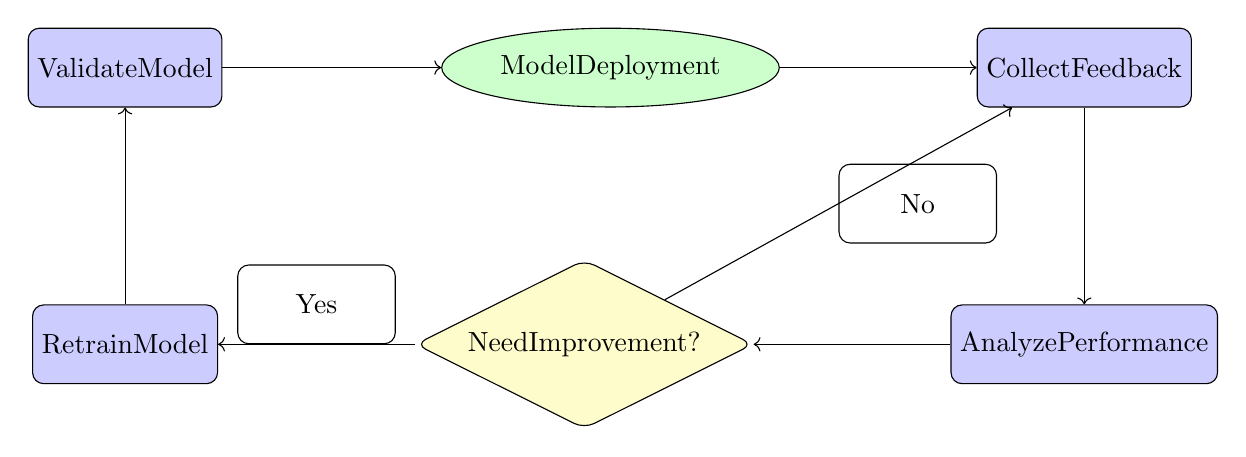
\begin{tikzpicture}[
    node distance=2.5cm,
    every node/.style={draw, rounded corners, minimum height=1cm, text centered, minimum width=2cm},
    start/.style={fill=green!20, ellipse},
    process/.style={fill=blue!20},
    decision/.style={fill=yellow!20, diamond, aspect=2},
    end/.style={fill=red!20, ellipse}
]

\node[start] (start) {Model\\Deployment};
\node[process, right=of start] (collect) {Collect\\Feedback};
\node[process, below=of collect] (analyze) {Analyze\\Performance};
\node[decision, left=of analyze] (improve) {Need\\Improvement?};
\node[process, left=of improve] (retrain) {Retrain\\Model};
\node[process, above=of retrain] (validate) {Validate\\Model};

% Connections
\draw[->] (start) -- (collect);
\draw[->] (collect) -- (analyze);
\draw[->] (analyze) -- (improve);
\draw[->] (improve) -- node[above] {Yes} (retrain);
\draw[->] (retrain) -- (validate);
\draw[->] (validate) -- (start);
\draw[->] (improve) -- node[right] {No} (collect);

\end{tikzpicture}
\caption{Continuous Model Improvement Cycle}
\label{fig:improvement_cycle}
\end{figure}

\section{Performance Optimization Strategies}

\subsection{Model Compression}

To ensure fast inference times, the system employs various model compression techniques:

\begin{enumerate}
    \item \textbf{Knowledge Distillation}: Training smaller models to mimic larger, more complex models
    \item \textbf{Quantization}: Reducing model precision while maintaining accuracy
    \item \textbf{Pruning}: Removing less important connections in neural networks
\end{enumerate}

\subsection{Caching Strategy}

A multi-level caching system optimizes response times:

\begin{figure}[H]
\centering
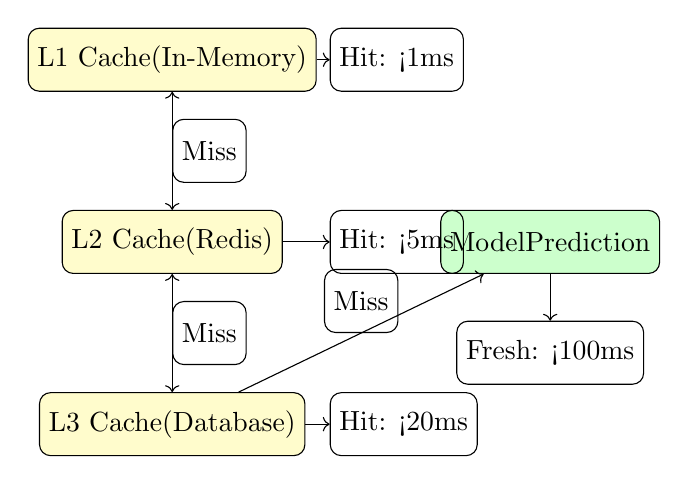
\begin{tikzpicture}[
    node distance=1.5cm,
    every node/.style={draw, rounded corners, minimum height=0.8cm, text centered},
    cache/.style={fill=yellow!20},
    process/.style={fill=green!20}
]

\node[cache] (l1) {L1 Cache\\(In-Memory)};
\node[cache, below=of l1] (l2) {L2 Cache\\(Redis)};
\node[cache, below=of l2] (l3) {L3 Cache\\(Database)};
\node[process, right=2cm of l2] (prediction) {Model\\Prediction};

% Cache hierarchy
\draw[<->] (l1) -- node[right] {Miss} (l2);
\draw[<->] (l2) -- node[right] {Miss} (l3);
\draw[->] (l3) -- node[above] {Miss} (prediction);

% Hit paths
\draw[->] (l1) -- ++(2,0) node[right] {Hit: <1ms};
\draw[->] (l2) -- ++(2,0) node[right] {Hit: <5ms};
\draw[->] (l3) -- ++(2,0) node[right] {Hit: <20ms};
\draw[->] (prediction) -- ++(0,-1) node[below] {Fresh: <100ms};

\end{tikzpicture}
\caption{Multi-Level Caching Strategy}
\label{fig:caching_strategy}
\end{figure}

\section{Security and Privacy Considerations}

The predictive analytics system implements comprehensive security measures:

\subsection{Data Protection}

\begin{enumerate}
    \item \textbf{Encryption}: All data is encrypted at rest and in transit
    \item \textbf{Access Control}: Role-based access to sensitive model data
    \item \textbf{Anonymization}: Personal identifiers are removed from training data
    \item \textbf{Differential Privacy}: Statistical noise added to protect individual privacy
\end{enumerate}

\subsection{Model Security}

\begin{figure}[H]
\centering
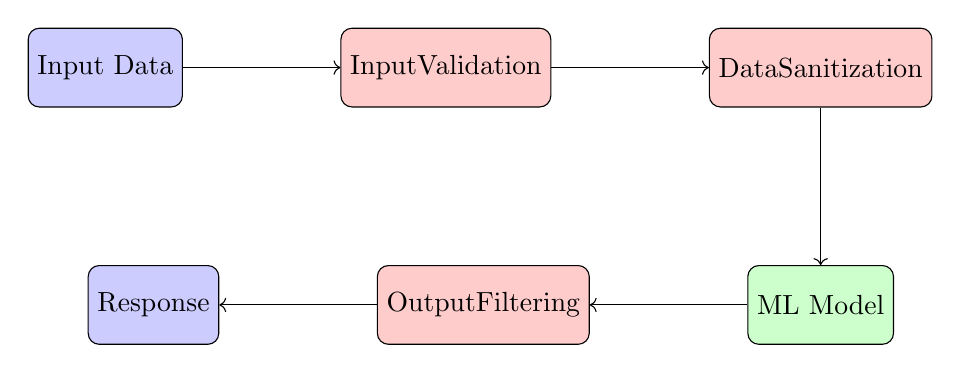
\begin{tikzpicture}[
    node distance=2cm,
    every node/.style={draw, rounded corners, minimum height=1cm, text centered},
    input/.style={fill=blue!20},
    security/.style={fill=red!20},
    process/.style={fill=green!20}
]

\node[input] (data_input) {Input Data};
\node[security, right=of data_input] (validation) {Input\\Validation};
\node[security, right=of validation] (sanitization) {Data\\Sanitization};
\node[process, below=of sanitization] (model) {ML Model};
\node[security, left=of model] (output_filter) {Output\\Filtering};
\node[input, left=of output_filter] (response) {Response};

\draw[->] (data_input) -- (validation);
\draw[->] (validation) -- (sanitization);
\draw[->] (sanitization) -- (model);
\draw[->] (model) -- (output_filter);
\draw[->] (output_filter) -- (response);

\end{tikzpicture}
\caption{Security Pipeline for Model Inference}
\label{fig:security_pipeline}
\end{figure}

\section{Future Enhancements}

\subsection{Advanced Learning Techniques}

Future versions will incorporate:

\begin{enumerate}
    \item \textbf{Reinforcement Learning}: Learning optimal estimation strategies through trial and error
    \item \textbf{Transfer Learning}: Applying knowledge from similar domains to improve accuracy
    \item \textbf{Federated Learning}: Training models across distributed datasets while preserving privacy
    \item \textbf{Meta-Learning}: Learning to learn from limited data for new project types
\end{enumerate}

\subsection{Integration Roadmap}

\begin{figure}[H]
\centering
\begin{tikzpicture}[
    node distance=2cm,
    every node/.style={draw, rounded corners, minimum height=1cm, text centered},
    current/.style={fill=green!20},
    planned/.style={fill=blue!20},
    future/.style={fill=orange!20}
]

% Timeline
\draw[thick] (0,0) -- (12,0);
\foreach \x/\label in {0/Q1, 3/Q2, 6/Q3, 9/Q4, 12/Q5} {
    \draw (\x,0.1) -- (\x,-0.1);
    \node[below] at (\x,-0.3) {\label};
}

% Current features
\node[current, above=0.5cm of 1.5cm] (ensemble) {Ensemble\\Models};

% Planned features
\node[planned, above=1.5cm of 4.5cm] (rl) {Reinforcement\\Learning};
\node[planned, above=0.5cm of 4.5cm] (transfer) {Transfer\\Learning};

% Future features
\node[future, above=1.5cm of 7.5cm] (federated) {Federated\\Learning};
\node[future, above=0.5cm of 7.5cm] (meta) {Meta\\Learning};

\node[future, above=1.5cm of 10.5cm] (quantum) {Quantum ML\\Integration};

\end{tikzpicture}
\caption{Machine Learning Enhancement Roadmap}
\label{fig:roadmap}
\end{figure}

\section{Conclusion}

The TaskWeight predictive analytics system represents a significant advancement in intelligent project management tools. By leveraging cutting-edge machine learning techniques, the system provides accurate, personalized task estimations that improve over time. The architecture's emphasis on explainability, security, and scalability ensures that it can meet the demands of modern software development teams while maintaining user trust and system reliability.

The continuous learning capabilities, combined with the ensemble approach and real-time processing, create a robust foundation for accurate task estimation. As the system evolves, the integration of advanced techniques such as reinforcement learning and federated learning will further enhance its capabilities, making TaskWeight an indispensable tool for project management in the digital age.

The success of this predictive analytics system lies not only in its technical sophistication but also in its practical applicability to real-world project management challenges. By providing transparent, accurate, and continuously improving estimates, TaskWeight empowers development teams to make better decisions, improve planning accuracy, and ultimately deliver more successful projects.

\bibliographystyle{plain}
\begin{thebibliography}{9}

\bibitem{chen2019}
Chen, T., \& Guestrin, C. (2016). XGBoost: A scalable tree boosting system. \emph{Proceedings of the 22nd ACM SIGKDD International Conference on Knowledge Discovery and Data Mining}, 785-794.

\bibitem{hochreiter1997}
Hochreiter, S., \& Schmidhuber, J. (1997). Long short-term memory. \emph{Neural Computation}, 9(8), 1735-1780.

\bibitem{lundberg2017}
Lundberg, S. M., \& Lee, S. I. (2017). A unified approach to interpreting model predictions. \emph{Advances in Neural Information Processing Systems}, 30, 4765-4774.

\bibitem{breiman2001}
Breiman, L. (2001). Random forests. \emph{Machine Learning}, 45(1), 5-32.

\bibitem{wolpert1992}
Wolpert, D. H. (1992). Stacked generalization. \emph{Neural Networks}, 5(2), 241-259.

\bibitem{vaswani2017}
Vaswani, A., Shazeer, N., Parmar, N., Uszkoreit, J., Jones, L., Gomez, A. N., ... \& Polosukhin, I. (2017). Attention is all you need. \emph{Advances in Neural Information Processing Systems}, 30, 5998-6008.

\bibitem{dwork2006}
Dwork, C. (2006). Differential privacy. \emph{33rd International Colloquium on Automata, Languages and Programming}, 1-12.

\bibitem{mcmahan2017}
McMahan, B., Moore, E., Ramage, D., Hampson, S., \& y Arcas, B. A. (2017). Communication-efficient learning of deep networks from decentralized data. \emph{Artificial Intelligence and Statistics}, 1273-1282.

\bibitem{finn2017}
Finn, C., Abbeel, P., \& Levine, S. (2017). Model-agnostic meta-learning for fast adaptation of deep networks. \emph{International Conference on Machine Learning}, 1126-1135.

\end{thebibliography}

\end{document}
